\documentclass[conference]{IEEEtran}
\usepackage{cite}
\usepackage{amsmath,amssymb,amsfonts}
\usepackage{graphicx}
\usepackage{booktabs}
\usepackage{xcolor}
\usepackage{url}
\usepackage{multirow}

\graphicspath{{Images/}{./}}

\def\BibTeX{{\rm B\kern-.05em{\sc i\kern-.025em b}\kern-.08em
    T\kern-.1667em\lower.7ex\hbox{E}\kern-.125emX}}

\begin{document}

\title{Exact Design-Space Exploration for SoC Security Feature Synthesis: A Declarative Formulation with Cross-Solver Validation on OpenTitan}

\author{\IEEEauthorblockN{Anonymous Submission}}

\maketitle

\begin{abstract}
Security features in Systems-on-Chip consume the same LUT, FF, power,
and latency budget as the functional design, yet security architecture
decisions are still made manually. This paper formulates system-level
security feature synthesis as an exact constrained optimization
problem using Answer Set Programming (ASP). Given a component and asset
model with impact annotations, the method selects a security mechanism
and a monitoring option for every component under explicit FPGA resource
and per-asset latency constraints, returning provably optimal solutions.

We validate on a benchmark suite spanning 1 to 20
components across 27 runs. The largest case is a 20-component
instance derived from the open-source OpenTitan Earl Grey
root-of-trust SoC, targeting a Xilinx Kintex-7 410T FPGA. To
establish correctness independently of the ASP solver, an equivalent
Constraint Programming (CP-SAT) formulation is built and
cross-validated: all 24 synthetic runs (1--8~components) produce
identical proven-optimal objectives across both solvers, providing
strong evidence of formulation correctness. At 20~components, ASP does not converge to
the proven optimum within a 120\,s timeout, while CP-SAT proves optimality in
under 0.1\,s, revealing a qualitative scalability boundary that motivates a
hybrid workflow. The benchmark demonstrates constraint sensitivity at
realistic scale: latency constraints alone force three high-impact
components off zero-trust; tightening LUTs raises risk from 1{,}804
to 3{,}449 ($1.91\times$); restricting power forces a mixed
security assignment exploiting redundancy-group structure.
Greedy and local-search heuristics using the same objective match the
optimum under two profiles but miss by 5\% under the tightest.
\end{abstract}

\begin{IEEEkeywords}
design-space exploration, security-aware CAD, System-on-Chip, Answer Set
Programming, FPGA, feature synthesis, OpenTitan, cross-solver validation
\end{IEEEkeywords}

%===================================================================
\section{Introduction}
%===================================================================

Modern SoCs integrate processors, accelerators, memories, and
peripherals on a shared interconnect. A security decision at one
component (selecting a zero-trust firewall versus a
lightweight MAC checker, for instance) affects system-wide risk exposure,
implementation cost, and timing across the device. This makes
security architecture a constrained optimization problem: security
features, anomaly detectors, and bus monitors improve protection but
consume the same LUT, FF, power, and latency budget needed by the
functional design.

Prior work has argued that security should become a first-class
design objective in embedded-system
exploration~\cite{pimentel_case_2020}, and several papers have
explored design-for-security tradeoffs for specific vulnerabilities or
application domains~\cite{stierand_integrating_2014,
liu_hardware_2015, rajmohan_hybrid_2020, gressl_security_2019,
gressl_design_2021, linares_design_2021, mahfuz_x-dfs_2025}. What is
still missing is (i)~a clean, implementation-aware formulation for
\emph{system-level} feature synthesis solved to proven optimality,
(ii)~cross-solver validation establishing that the reported optima are
correct, and (iii)~evaluation on an architecture-realistic benchmark
derived from an open-source SoC at a scale that reveals design
insights invisible in small synthetic cases.

We address all three gaps. We formulate security feature synthesis
in ASP and solve it with clingo~\cite{gebser_potassco_2011}. To
validate the results independently, we build an equivalent CP-SAT
formulation using Google OR-Tools~\cite{ortools} and cross-validate
on every benchmark instance. Our benchmark suite
includes eight synthetic cases (1--8 components) and a 20-component
instance derived from OpenTitan Earl Grey~\cite{opentitan_repo}, an
open-source silicon root-of-trust SoC with cryptographic accelerators,
a key manager, lifecycle controller, and communication peripherals.

Our contributions are fourfold:
\begin{enumerate}
\item An exact formulation of system-level SoC security feature
synthesis under explicit LUT, FF, power, and per-asset latency
constraints, expressed in ASP and solved with clingo.
\item Cross-solver validation: an equivalent CP-SAT model produces
identical proven-optimal objectives on all 24 synthetic runs (1--8
components), providing strong evidence of formulation correctness independently of
the solver.
\item A scalability comparison from 1 to 20 components showing that
ASP proves optimality up to 8~components (2.85\,s mean) but fails at
20, while CP-SAT solves every case in under 0.1\,s, motivating a
hybrid workflow with CP-SAT as the production feature-synthesis solver.
\item A constraint-sensitivity finding on the 20-component OpenTitan
case: latency constraints force three components off zero-trust even
under full resources; tightening power further forces a mixed
9~ZT~+~7~DM~+~4~MAC assignment that exploits redundancy-group
structure; greedy and local-search heuristics using the same
redundancy-aware objective match the optimum under two profiles
but miss by 5\% under the tightest multi-constraint case.
\end{enumerate}

%===================================================================
\section{Related Work}
%===================================================================

Security-aware design-space exploration has been studied for over a
decade. In our reading of this literature, most existing work either
optimizes for a specific vulnerability or treats security as an
auxiliary constraint.
Stierand et al.~\cite{stierand_integrating_2014} integrated security
requirements into DSE but did not calibrate implementation costs.
Gressl et al.~\cite{gressl_security_2019, gressl_design_2021}
explored secure IoT alternatives derived from known attacks.
Liu and Li~\cite{liu_hardware_2015}, Rajmohan
et al.~\cite{rajmohan_hybrid_2020}, and Linares et
al.~\cite{linares_design_2021} each study narrower implementation
spaces around particular protections. Mahfuz
et al.~\cite{mahfuz_x-dfs_2025} use explainable AI for
design-for-security exploration, but target rule-guided hardening rather
than exact implementation-aware synthesis.

None of these works (i)~solve the system-level feature selection problem
to proven optimality under FPGA resource constraints, (ii)~provide
cross-solver validation of the reported optima, or (iii)~evaluate on an architecture-realistic benchmark derived
from an open-source SoC.

On the solver side, ASP has been used for hardware
configuration~\cite{gebser_potassco_2011} and combinatorial
optimization. CP-SAT~\cite{ortools} is a state-of-the-art constraint
programming solver. Using both on the same problem provides
solver-independent correctness evidence that is standard practice in
operations research but rare in security-aware CAD.

%===================================================================
\section{Problem Formulation}
%===================================================================

\subsection{System Model}

We model the input as a set of components $\mathcal{C}$, each containing
assets with declared read/write impact scores and per-asset latency caps.
Our synthesis engine assigns one security feature $s \in
\{$\texttt{mac}, \texttt{dynamic\_mac}, \texttt{zero\_trust}$\}$ and
one logging feature $\ell \in \{$\texttt{no\_logging},
\texttt{some\_logging}, \texttt{zero\_trust\_logger}$\}$ to each
component. Each feature pair $(s, \ell)$ has known LUT, FF,
power, and latency costs drawn from a Vivado-derived catalog, as well as
vulnerability ($V$) and logging ($L$) scores that determine residual
risk.

\subsection{Feature Catalog}

We derive feature costs from Vivado~2023.x synthesis of standalone
security IP cores (a MAC checker, a dynamic-MAC engine with nonce
management, a zero-trust firewall, and three monitoring/logging
engines) targeting a Xilinx xc7z020 (PYNQ-Z2 class) at 125\,MHz.
Zero-trust resource estimates are based on possible implementations
explored in Butka and Bobda~\cite{butka_measuring_2025}. LUT and FF counts
are architecture-independent 7-series primitive counts and transfer
directly to XC7K410T without correction. Power values are Vivado
static-power estimates normalised to $10^{-2}$\,W integers; they are
order-of-magnitude indicators, not post-place-and-route measurements.
The zero-trust logger's large base cost (31{,}354~LUTs) reflects a
full transaction-logging engine with FIFO and formatter.

Each feature has three cost tiers:
a \emph{per-asset} cost (proportional to the number of assets on the
component), a \emph{per-component} cost (fixed per protected component),
and a \emph{base} cost (one-time overhead, shared across all components
using that feature). Table~\ref{tab:catalog} summarizes the catalog.

\begin{table}[t]
\caption{Feature-cost catalog (Vivado synthesis, xc7z020 @ 125\,MHz)}
\label{tab:catalog}
\centering
\resizebox{\columnwidth}{!}{%
\scriptsize
\setlength{\tabcolsep}{2.5pt}
\begin{tabular}{llrrrrrrrr}
\toprule
Feature & Class & \multicolumn{3}{c}{LUTs} & \multicolumn{3}{c}{FFs} & $V$ / $L$ & Pwr$^a$ \\
\cmidrule(lr){3-5}\cmidrule(lr){6-8}
& & /asset & /comp & base & /asset & /comp & base & & \\
\midrule
MAC             & sec &  51 & 234 &    0 &  32 & 292 &    0 & $V\!=\!30$ & 2 \\
Dynamic MAC     & sec &  51 & 234 & 1985 &  32 & 292 & 1612 & $V\!=\!20$ & 2 \\
Zero Trust      & sec &  90 & 380 & 3200 &  56 & 480 & 2600 & $V\!=\!10$ & 3 \\
ZT Logger       & log & --- & --- & 31354& --- & --- & 25020& $L\!=\!5$ & 717 \\
Some Logging    & log & --- & --- & 3135 & --- & --- & 2502 & $L\!=\!10$ & 72 \\
No Logging      & log & --- & --- &    0 & --- & --- &    0 & $L\!=\!20$ & 0 \\
\bottomrule
\multicolumn{10}{l}{\scriptsize Base costs are shared across components that use the same feature.} \\
\multicolumn{10}{l}{\scriptsize $^a$Power ($10^{-2}$\,W): byAsset + byComponent + base for security; base-only for logging.}
\end{tabular}}
\end{table}

Lower $V$ and $L$ scores reduce residual risk (Eq.~\ref{eq:risk}), but
stronger features cost more resources. Vulnerability scores are scaled
by~10 ($V\!=\!10,20,30$) to keep all arithmetic in integers.
Zero-trust provides the lowest vulnerability ($V\!=\!10$) but requires
more LUTs, FFs, and power per component than MAC or dynamic-MAC
(Table~\ref{tab:catalog}), creating a genuine cost--security tradeoff
that the optimizer must resolve under each constraint profile. The
zero-trust logger, with $L=5$, cuts the logging factor $4\times$
relative to no-logging ($L=20$), but at a base cost of 31{,}354~LUTs.
Whether these tradeoffs are worthwhile depends on the system's impact
distribution and resource budget; the optimizer answers these
questions automatically.

\subsection{Risk Objective}

For each component $c$, asset $a$, and operation $op$, residual risk
follows the multiplicative model of Butka and
Bobda~\cite{butka_measuring_2025}:
\begin{equation}
r(c,a,op)=\left\lfloor \frac{I(a,op)\cdot V(s_c)\cdot L(\ell_c)}{10}\right\rfloor
\label{eq:risk}
\end{equation}
where $I$ is the declared impact (1--10), $V$ is the vulnerability score
of the selected security feature $s_c$ ($V\!=\!10,20,30$; lower is
better), and $L$ is the logging score ($L\!=\!5,10,20$; lower is
better). Both $V$ and $L$ are scaled by~10 for integer arithmetic;
the divisor compensates, giving effective risk multipliers in
$[5,\,60]$.

The multiplicative form follows the standard risk = impact $\times$
likelihood decomposition (ISO~27005, NIST SP~800-30): $V$ quantifies
residual exposure after the selected prevention mechanism, and $L$
quantifies residual observability gap (a component with full logging has
lower undetected-compromise likelihood). The product $V \cdot L$
serves as a proxy for residual likelihood given the chosen feature pair, and
multiplication with $I$ yields a composite risk score. We treat
$V$ and $L$ as interval-scaled design parameters proportional to
residual exposure, giving an \emph{engineering scoring heuristic}
suitable for comparative optimization across feature assignments.
A per-asset risk cap $r(c,a,op) \leq R_{\max}$ ensures no single
asset exceeds an acceptable threshold.

Our objective minimizes total system risk:
\begin{equation}
\min \sum_{c,a,op} r(c,a,op)
\end{equation}
subject to per-resource constraints (LUTs, FFs, power),
per-asset latency caps, and the per-asset risk cap.

\subsection{OpenTitan Earl Grey Benchmark}

To move beyond synthetic architectures, we derive a 20-component
benchmark from the OpenTitan Earl Grey~\cite{opentitan_repo}
architecture, an open-source silicon root-of-trust SoC designed by
lowRISC. Our component set (Table~\ref{tab:otmap}) maps one-to-one
with Earl Grey IP blocks. We assigned impact scores to reflect each
block's architectural criticality: cryptographic engines and the key
manager receive the highest scores; communication peripherals the
lowest.
Latency caps reflect each block's timing criticality: the Ibex
processor, DMA controller, and key manager require 5-cycle access
(forcing MAC), while crypto accelerators allow 7--10 cycles and
peripherals are relaxed to 50--1000.
The benchmark is
``architecture-derived'': it preserves OpenTitan's component
topology and role differentiation but relies on the external
security-IP cost catalog (Table~\ref{tab:catalog}), not on OpenTitan's
actual gate-level implementations.

\begin{table}[t]
\caption{OpenTitan Earl Grey component mapping (20 IPs)}
\label{tab:otmap}
\centering
\scriptsize
\setlength{\tabcolsep}{2.5pt}
\begin{tabular}{llrrl}
\toprule
Comp. & OpenTitan IP & $I_r$ & $I_w$ & Role \\
\midrule
cpu    & Ibex RISC-V     & 10 & 10 & Master processor \\
dma    & DMA controller  &  8 &  8 & Bus master \\
aes    & AES accelerator &  9 & 10 & Symmetric crypto \\
hmac   & HMAC            &  8 &  9 & Authentication \\
kmac   & KMAC            &  8 &  9 & Keccak MAC \\
otbn   & OTBN bignum     &  9 & 10 & Asymmetric crypto \\
keymgr & Key manager     & 10 & 10 & Root of trust \\
otp    & OTP controller  &  9 &  9 & Immutable fuses \\
lc     & Lifecycle ctrl  &  9 &  8 & State transitions \\
flash  & Flash ctrl      &  7 &  8 & Code/data storage \\
sram   & SRAM ctrl       &  5 &  6 & Working memory \\
rom    & ROM ctrl        &  6 &  3 & Boot code \\
uart0  & UART 0          &  3 &  3 & Serial I/O \\
uart1  & UART 1          &  3 &  3 & Serial I/O \\
gpio   & GPIO            &  2 &  4 & General I/O \\
spi    & SPI host        &  4 &  5 & SPI interface \\
i2c    & I2C             &  3 &  4 & I2C interface \\
timer  & Timer           &  2 &  2 & Non-critical \\
alert  & Alert handler   &  7 &  5 & Security monitor \\
entropy& Entropy source  &  8 &  7 & RNG + health \\
\bottomrule
\end{tabular}
\end{table}

Two redundancy groups model defense-in-depth coverage:
AES/HMAC/KMAC (crypto accelerators that jointly protect
key material, so compromise of one does not expose data protected by
the others) and UART0/UART1 (redundant communication channels).
Group membership asserts overlapping security coverage: combined residual
exposure is lower than any single member's.

\subsection{Redundancy Model}
\label{sec:redun}

For components not in any group, risk follows Eq.~\ref{eq:risk}
directly. For components in a redundancy group~$G = \{c_1, \ldots,
c_n\}$, the formulation combines per-member residual probabilities
before computing risk, modelling independent exposure reduction.

Each member's $V \cdot L$ product is normalised to a common scale
using parameters $\mu\!=\!25$ (floor) and $\omega\!=\!1000$ (ceiling):
\begin{equation}
p_{\text{norm}}(c) = \frac{(V_c \cdot L_c - \mu) \cdot 1000}{\omega - \mu}
\label{eq:norm}
\end{equation}
The combined normalised probability is the recursive product:
\begin{equation}
P_G = \frac{p_{\text{norm}}(c_1) \cdot p_{\text{norm}}(c_2) \cdots p_{\text{norm}}(c_n)}{1000^{\,n-1}}
\label{eq:combine}
\end{equation}
which is then denormalised back:
$p_{\text{denorm}} = P_G \cdot (\omega - \mu) / 1000 + \mu \cdot 10$.
Group-member risk becomes
$r(c,a,op) = \lfloor I(a,op) \cdot p_{\text{denorm}} / 100 \rfloor$.
The $1000^{n-1}$ divisor ensures that adding a redundant member always
reduces combined risk, thus giving the optimizer an incentive to accept
weaker per-member security when the group already provides coverage.

%===================================================================
\section{Solver Formulations}
%===================================================================

\subsection{ASP Formulation}

We encode the problem in ASP and solve it with clingo
5.8.0~\cite{gebser_potassco_2011}. Each component receives exactly one
security and one logging feature:
\begin{equation}
\sum_{s \in F_{\text{sec}}} \text{sel\_sec}(c,s)=1,\quad
\sum_{\ell \in F_{\text{log}}} \text{sel\_log}(c,\ell)=1
\end{equation}

Hard constraints enforce device budgets:
\begin{equation}
\text{LUTs}_{\text{used}}\leq \text{LUTs}_{\max},\quad
\text{Power}_{\text{used}}\leq \text{Power}_{\max}
\end{equation}
\begin{equation}
\forall(c,a,op): \; \text{latency}(s_c)\leq \text{cap}(a,op)
\end{equation}
The latency constraint checks only the security feature's cycle cost;
logging operates asynchronously and does not add cycles to the
protected access path.

Our objective minimizes total residual risk under these constraints.
The ASP encoding is declarative: adding a new security feature requires
only adding catalog facts, not modifying the solver logic. In our view,
this extensibility is the primary reason to choose ASP over imperative
formulations.

\subsection{CP-SAT Formulation}

To validate the ASP results independently, an equivalent model is built
using Google OR-Tools CP-SAT~\cite{ortools}. The CP-SAT model uses:
\begin{itemize}
\item \textbf{Element constraints} to look up per-pair (security $\times$
logging) resource costs and $V \cdot L$ products from precomputed tables.
\item \textbf{Multiplication and division equalities} to compute
$I \cdot V \cdot L / 10$ for each asset.
\item \textbf{Boolean indicators} with conditional constraints to track
one-time base costs for each feature used.
\end{itemize}

Both formulations encode the identical optimization problem. Any
objective mismatch would indicate a formulation error.

%===================================================================
\section{Experimental Setup}
%===================================================================

\subsection{Benchmark Suite}

Our suite contains nine instance families: eight synthetic cases (TC1--TC9,
excluding TC4, which uses a hierarchical component model with a different
arity than the flat \texttt{component/1} encoding shared by the remaining
cases and both solvers) and the OpenTitan-derived case (OT).
Table~\ref{tab:suite} summarizes the benchmark.

\begin{table}[t]
\caption{Benchmark suite}
\label{tab:suite}
\centering
\footnotesize
\begin{tabular}{lrrcc}
\toprule
Case & Comp. & Assets & Groups & Target \\
\midrule
TC1  &  3 &  3 & no  & Synthetic \\
TC2  &  8 &  8 & no  & Synthetic \\
TC3  &  1 &  8 & no  & Synthetic \\
TC5  &  8 &  8 & no  & Synthetic \\
TC6  &  3 &  3 & yes & Synthetic \\
TC7  &  8 &  8 & yes & Synthetic \\
TC8  &  8 &  8 & yes & Synthetic \\
TC9  &  8 &  8 & yes & Synthetic \\
\midrule
OT   & 20 & 20 & yes & OpenTitan Earl Grey \\
\bottomrule
\end{tabular}
\end{table}

\subsection{Constraint Profiles}

Each synthetic case is evaluated under three profiles
(Table~\ref{tab:profiles}) targeting a Xilinx
xc7z020 (PYNQ-Z2). The OpenTitan case uses three profiles targeting a
Xilinx Kintex-7 410T. OT-A provides full resources; OT-B restricts LUTs to
25{,}000 (below the 45{,}014 required by the OT-A optimum); OT-C
restricts power to 800 (below the 812 required by OT-A), forcing
the optimizer to substitute cheaper security features on some components.

\begin{table}[t]
\caption{Constraint profiles}
\label{tab:profiles}
\centering
\footnotesize
\begin{tabular}{llrrr}
\toprule
Profile & Target & LUT cap & Power cap & Risk cap \\
\midrule
A    & xc7z020  &  53,200 & 15,000 & 100 \\
B    & xc7z020  &  10,000 & 15,000 & 500 \\
C    & xc7z020  &  53,200 &  1,000 & 100 \\
\midrule
OT-A & XC7K410T & 254,200 & 15,000 & 200 \\
OT-B & XC7K410T &  25,000 & 15,000 & 500 \\
OT-C & XC7K410T & 254,200 &    800 & 200 \\
\bottomrule
\end{tabular}
\end{table}

\subsection{Experimental Environment}

Experiments ran on one P-core of an Intel Core i7-12700H (2.3\,GHz)
with 32\,GB RAM, Windows~11, Python~3.12, clingo~5.8.0, and
OR-Tools~9.x. Both solvers were run single-threaded for fair comparison.

%===================================================================
\section{Results}
\label{sec:results}
%===================================================================

\subsection{Cross-Solver Validation}

Table~\ref{tab:crossval} reports the complete benchmark results. All 24
synthetic runs (1--8 components) produce identical proven-optimal
objectives between ASP and CP-SAT, confirming that both formulations
encode the same optimization problem. At 20~components (OpenTitan),
CP-SAT proves optimality in under 0.1\,s, but ASP does not converge
to the proven optimum within its 120\,s timeout, confirming a
qualitative scalability boundary between 8 and 20~components.

\begin{table}[t]
\caption{Benchmark results: 24 cross-validated synthetic + 3 OpenTitan}
\label{tab:crossval}
\centering
\resizebox{\columnwidth}{!}{%
\scriptsize
\setlength{\tabcolsep}{2.5pt}
\begin{tabular}{lrrrrrl}
\toprule
Case & Comp. & Prof. & Obj. & ASP\,(s) & CP-SAT\,(s) & Match \\
\midrule
TC1 &  3 & A    &   90 & 0.125 & 0.010 & \checkmark \\
TC1 &  3 & B    &  180 & 0.116 & 0.006 & \checkmark \\
TC1 &  3 & C    &   90 & 0.117 & 0.005 & \checkmark \\
TC2 &  8 & A    &  365 & 2.424 & 0.007 & \checkmark \\
TC2 &  8 & B    &  860 & 3.616 & 0.011 & \checkmark \\
TC2 &  8 & C    &  365 & 2.579 & 0.007 & \checkmark \\
TC3 &  1 & A    &  720 & 0.002 & 0.001 & \checkmark \\
TC3 &  1 & B    & 1{,}440 & 0.001 & 0.001 & \checkmark \\
TC3 &  1 & C    &  720 & 0.001 & 0.001 & \checkmark \\
TC5 &  8 & A    &  365 & 2.424 & 0.006 & \checkmark \\
TC5 &  8 & B    &  860 & 3.436 & 0.011 & \checkmark \\
TC5 &  8 & C    &  365 & 2.559 & 0.007 & \checkmark \\
TC6 &  3 & A    &   45 & 0.107 & 0.015 & \checkmark \\
TC6 &  3 & B    &   45 & 0.101 & 0.012 & \checkmark \\
TC6 &  3 & C    &   45 & 0.134 & 0.018 & \checkmark \\
TC7 &  8 & A    &  232 & 2.534 & 0.021 & \checkmark \\
TC7 &  8 & B    &  402 & 3.226 & 0.023 & \checkmark \\
TC7 &  8 & C    &  232 & 2.530 & 0.015 & \checkmark \\
TC8 &  8 & A    &  331 & 2.538 & 0.010 & \checkmark \\
TC8 &  8 & B    &  761 & 3.337 & 0.017 & \checkmark \\
TC8 &  8 & C    &  331 & 2.537 & 0.010 & \checkmark \\
TC9 &  8 & A    &  219 & 2.821 & 0.016 & \checkmark \\
TC9 &  8 & B    &  364 & 3.337 & 0.024 & \checkmark \\
TC9 &  8 & C    &  219 & 3.098 & 0.018 & \checkmark \\
\midrule
OT  & 20 & OT-A &1{,}804 & $>$165$^\dagger$ & 0.05 & --- \\
OT  & 20 & OT-B &3{,}449 & $>$296$^\dagger$ & 0.05 & --- \\
OT  & 20 & OT-C &1{,}854 & $>$213$^\dagger$ & 0.05 & --- \\
\bottomrule
\multicolumn{7}{l}{\scriptsize $^\dagger$ASP suboptimal; objectives are CP-SAT proven optima.}
\end{tabular}}
\end{table}

\subsection{Scalability Analysis}

Table~\ref{tab:scale} aggregates solve time by component count.
At 1~component, both solvers finish in under 2\,ms. At
3~components, ASP takes 0.12\,s (dominated by grounding), while
CP-SAT stays under 12\,ms. At 8~components, ASP averages 2.85\,s
while CP-SAT remains under 25\,ms, a
$220\times$ speedup. At 20~components (OpenTitan), ASP does not
converge to the proven optimum within its timeout, while CP-SAT proves
optimality in under 0.1\,s. The scalability boundary between 8 and
20~components marks where CP-SAT becomes essential for practical use.

\begin{table}[t]
\caption{Scalability: mean solve time by component count}
\label{tab:scale}
\centering
\footnotesize
\begin{tabular}{rrrr}
\toprule
Components & ASP mean\,(s) & CP-SAT mean\,(s) & Ratio \\
\midrule
 1 &  0.001 & 0.001 & 1$\times$ \\
 3 &  0.12  & 0.012 & 10$\times$ \\
 8 &  2.85  & 0.013 & 220$\times$ \\
20 & $>$225$^\dagger$ & 0.05 & $>$4{,}500$\times$ \\
\bottomrule
\multicolumn{4}{l}{\scriptsize $^\dagger$ASP did not prove optimality; best-found was suboptimal.}
\end{tabular}
\end{table}

Figure~\ref{fig:runtime} plots the scaling trend on a log scale. The gap
between solvers widens steadily: $1\times$ at 1~component,
$10\times$ at~3, $220\times$ at~8, and $>$4{,}500$\times$ at~20
where ASP fails to prove optimality entirely. For rapid parameter
sweeps or larger designs, we recommend CP-SAT as the
feature-synthesis solver; ASP's value lies in the declarative
extensibility needed by downstream reasoning stages
(Section~\ref{sec:whyasp}).

\begin{figure}[t]
    \centering
    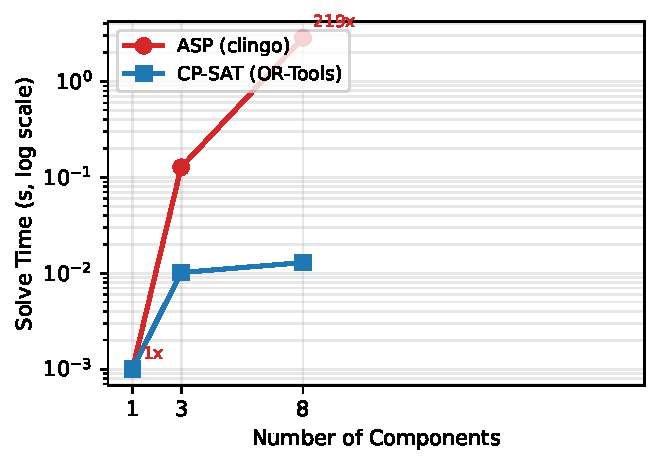
\includegraphics[width=0.95\columnwidth]{Images/runtime_scaling.pdf}
    \caption{Mean solve time vs.\ component count (log scale). The gap
    widens from $1\times$ at 1~component to $>$4{,}500$\times$ at
    20~components, where ASP cannot prove optimality.}
    \label{fig:runtime}
\end{figure}

\subsection{OpenTitan Design Insights}

Table~\ref{tab:ot_results} reports the OpenTitan results in detail.

\begin{table}[t]
\caption{OpenTitan Earl Grey results (20 components, CP-SAT proven optima)}
\label{tab:ot_results}
\centering
\footnotesize
\setlength{\tabcolsep}{3pt}
\begin{tabular}{lrrrll}
\toprule
Profile & Obj. & LUTs & Power & Security mix & Logging mix \\
\midrule
OT-A & 1{,}804 & 45{,}014 & 812 & 15\,ZT+2\,DM+3\,MAC & 20\,ZTL \\
OT-B & 3{,}449 & 16{,}610 & 165 & 14\,ZT+3\,DM+3\,MAC & 20\,SL \\
OT-C & 1{,}854 & 43{,}904 & 800 & 9\,ZT+7\,DM+4\,MAC & 20\,ZTL \\
\bottomrule
\end{tabular}
\vspace{2pt}
\scriptsize ZT=Zero Trust, DM=Dynamic MAC, MAC=MAC, ZTL=ZT Logger, SL=Some Logging
\end{table}

Under Profile~OT-A (full resources), latency constraints already
force the optimizer to differentiate: cpu, dma, and keymgr have
5-cycle latency caps that exclude zero-trust (8~cycles), so they
receive MAC; aes and otbn have 7-cycle caps that exclude ZT but
allow dynamic-MAC.  The remaining 15~components receive zero-trust.
Risk is~1{,}804 at 45{,}014~LUTs and 812~power.  Even with
non-binding resource budgets, latency alone prevents a uniform ZT
assignment.

Under OT-B (LUT cap 25{,}000), the ZTL base cost (31{,}354~LUTs)
exceeds the budget, so the optimizer switches all logging to
some-logging.  Latency constraints still force cpu/dma/keymgr to MAC,
and hmac joins the dynamic-MAC group.  Risk rises to~3{,}449.

The most interesting result is OT-C (power capped at 800).  Here the
optimizer must navigate power constraints, latency constraints, and
redundancy structure simultaneously.  It maintains full ZTL logging
but downgrades security on 11 of 20~components: 4~receive MAC and
7~receive dynamic-MAC, raising risk to~1{,}854.
Surprisingly, the three crypto accelerators (aes, hmac, kmac) all
receive dynamic-MAC or MAC despite their high individual impact.
Their redundancy group membership reduces combined probability enough
that ZT's risk saving is less valuable than the power saved by a
weaker feature.  Under OT-C's power pressure, the optimizer
downgrades crypto engines to exploit redundancy coverage rather than
spending the power budget on ZT for components whose group membership
already reduces combined risk.  This multi-constraint coordination
is where exact optimization adds the most value.

\begin{figure}[t]
    \centering
    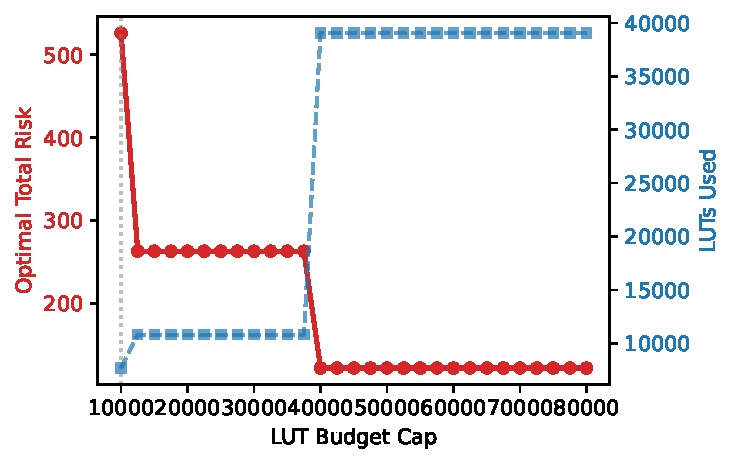
\includegraphics[width=0.95\columnwidth]{Images/pareto_sweep.pdf}
    \caption{Pareto sweep: optimal risk vs.\ LUT budget cap on the
    OpenTitan case.  Sharp transitions correspond to security-tier
    thresholds (all-MAC $\to$ DM mix $\to$ ZT mix);
    mixed security assignments appear under tight budgets.}
    \label{fig:pareto}
\end{figure}

\subsection{Heuristic Baseline Comparison}

To quantify what exactness buys, Table~\ref{tab:greedy}
compares CP-SAT optima against two heuristic baselines:
a \emph{greedy} heuristic that processes components by descending impact
and assigns the best affordable feature, and a \emph{local-search}
(1-opt) refinement that starts from the greedy solution and iteratively
swaps one component's security/logging assignment to the best feasible
improving neighbour until no single-component swap reduces risk.

\begin{table}[t]
\caption{Heuristic vs.\ optimal (CP-SAT) on OpenTitan profiles}
\label{tab:greedy}
\centering
\footnotesize
\begin{tabular}{lrrrrr}
\toprule
Profile & Optimal & Greedy & Gap$_G$ & Local-S & Gap$_{LS}$ \\
\midrule
OT-A & 1{,}804 & 1{,}804 & 0\% & 1{,}804 & 0\% \\
OT-B & 3{,}449 & 3{,}449 & 0\% & 3{,}449 & 0\% \\
OT-C & 1{,}854 & 1{,}948 & +5\% & 1{,}948 & +5\% \\
\bottomrule
\end{tabular}
\end{table}

Both heuristics use the same redundancy-aware objective as CP-SAT
(Section~\ref{sec:redun}), so the comparison is apples-to-apples.
The greedy assigns the lowest-risk latency-feasible pair to each
component in descending impact order, checking resource caps
incrementally.  Local search (1-opt) then swaps one component at a
time to the best feasible neighbour.

Under OT-A and OT-B, both heuristics match the proven optimum:
the greedy's impact-ordered processing happens to find the same
assignment the solver proves optimal.  Under OT-C, the gap is 5\%:
the simultaneous power and latency pressure creates a
multi-component coordination problem where the greedy's sequential
decisions cannot find the globally optimal trade between
crypto-group coverage and power savings.

\subsection{Perturbation Stability}

All 24 synthetic runs produce identical proven optima across ASP and
CP-SAT, validating the formulation on 1--8~component instances.
Profile~C always reproduces Profile~A at 8~components (power is never
binding), whereas on OpenTitan, OT-C produces a dramatically
different solution with mixed security assignments. Power sensitivity
and cost differentiation emerge only at realistic scale.

%===================================================================
\section{Discussion}
%===================================================================

\subsection{Why ASP for Security Feature Synthesis}
\label{sec:whyasp}

At 8~components CP-SAT is $220\times$ faster than ASP; at
20~components ASP cannot prove optimality at all, while CP-SAT
completes in under 0.1\,s (Table~\ref{tab:scale}). For
feature-synthesis alone, CP-SAT is the production solver.
ASP's value rests on the downstream reasoning stages.
Feature synthesis is the first of three stages; the maintained
repository also implements \emph{access-control policy synthesis}
(firewall placement, least-privilege gap analysis via
negation-as-failure) and \emph{resilience analysis}
(parallel transitive closures over degraded topologies,
bounded-depth attack-path enumeration). Both stages rely on
recursive reachability, negation-as-failure, and multi-level
implication chains, patterns natural in ASP but costly in CP-SAT
or ILP. A hybrid workflow makes sense: CP-SAT for
feature-synthesis optimization, ASP for the downstream stages.

\subsection{Relation to ILP/MIP Solvers}

The resource constraints are linear and the objective can be
linearised, so ILP solvers (e.g.\ Gurobi~\cite{gurobi}) could solve
the same problem. We chose CP-SAT because it is open-source and its
element constraints map naturally to feature selection; an ILP
comparison remains future work.

\subsection{Constraint Sensitivity as a Design Tool}

We see the OT results as a practical demonstration of exact DSE's
value: quantifying the security cost of constraint interactions.
Even under full resources (OT-A), latency alone raises risk from a
hypothetical all-ZT floor to~1{,}804 by forcing three components to
MAC.  Restricting LUTs to 25{,}000 (OT-B) eliminates ZTL logging
and tightens the security mix further, pushing risk to~3{,}449.
Power at 800~units (OT-C) forces a different trade: the optimizer
keeps ZTL but downgrades security on 11~components to a
9~ZT~+~7~DM~+~4~MAC mix at risk~1{,}854.  The Pareto sweep
(Figure~\ref{fig:pareto}) provides a complete risk--resource tradeoff
map.  Quantitative what-if analysis at this level is most reliable with an
exact solver that reports provably optimal solutions under each
constraint set; the greedy's 0\% gap on OT-A/OT-B shows that simpler
methods suffice when few constraints bind, but the 5\% gap on OT-C
illustrates the cost of sequential decision-making under tight
multi-constraint pressure.

\subsection{Limitations}

We assigned impact scores based on architectural criticality, not
measured vulnerability data. Our feature catalog comes from Vivado
synthesis of standalone security IP cores (MAC checker, dynamic-MAC
engine, zero-trust firewall, and three logging monitors), not the
actual OpenTitan blocks. The formulation
covers the feature-synthesis stage; the policy and resilience
stages are implemented in the maintained repository.
Scaling beyond 20~components to 50--100 component SoCs remains future
work.

%===================================================================
\section{Conclusion}
%===================================================================

We set out to answer a straightforward question: can security
feature synthesis for SoCs be solved exactly, and does exactness
actually matter compared to reasonable heuristics? The answer to both
is yes, but the path taught us more than the destination.

Cross-validating ASP against CP-SAT on 24 synthetic runs gave us
confidence that the formulation is correct, not just that one solver
happens to find good solutions.  The sharp divergence at 20 components was
informative. We now view CP-SAT as the right production solver for
feature synthesis, while ASP earns its keep in the downstream
policy and resilience stages where recursive reasoning dominates.

The result we find most valuable is how latency and power interact.
Under OT-A, latency alone forces cpu, dma, and keymgr off
zero-trust, producing a heterogeneous assignment even with non-binding resource budgets.  Under OT-C, adding a power constraint forces the
optimizer to downgrade 11 of 20 components, producing a
9\,ZT~+~7\,DM~+~4\,MAC mix where the crypto accelerators receive
weaker features because redundancy coverage absorbs the risk.
The greedy heuristic matches on OT-A and OT-B but misses by 5\%
on OT-C, where the power-latency interaction requires multi-component
coordination that sequential assignment cannot achieve.

Looking ahead, we plan to co-optimize firewall and policy placement
with feature selection, evaluate resilience under component-compromise
scenarios on the OpenTitan topology, and add an ILP solver as a
third comparison point.

Our ASP solver, CP-SAT benchmark, feature catalog, and all
benchmark instances are available in the accompanying
repository.\footnote{Repository URL withheld for double-blind review.}

\bibliographystyle{IEEEtran}
\bibliography{iccad_refs}

\end{document}
